
\documentclass[10pt,sans,english,compress,xcolor=dvipsnames]{beamer}



\author[Lily ]{ Dr Lily Asquith (Lily, she/her)}

\usetheme{Szeged}
%\defbeamertemplateparent{enumerate items}{enumerate item,enumerate subitem,enumerate subsubitem,enumerate mini template}
\definecolor{titcol}{RGB}{16,78,100} 
\setbeamercolor{frametitle}{fg=titcol,bg=White}
\useoutertheme{miniframes} 
\useinnertheme{rectangles}

\usepackage{pifont}
\newcommand{\tick}{\textcolor{grn}{\ding{52} } }
\newcommand{\nope}{\textcolor{red}{\ding{54} } }


\usepackage{soul}
\usepackage{cancel}

\usepackage[most]{tcolorbox}
\definecolor{LilyBlack}{rgb}{0.05,0.1,0.3} % UBC Blue (primary)
\usecolortheme[named=LilyBlack]{structure}

\usepackage{booktabs}
\usepackage{tabularx}
%\usepackage{tikz}
%\def\checkmark{\tikz\fill[scale=0.4](0,.35) -- (.25,0) -- (1,.7) -- (.25,.15) -- cycle;}

\usepackage{physics}

\usepackage{xparse}

\setbeamertemplate{footline}{%
  \leavevmode%
  \hbox{\begin{beamercolorbox}[wd=.5\paperwidth,ht=2.5ex,dp=1.125ex,leftskip=.3cm plus1fill,rightskip=.3cm]{author in head/foot}%
    \usebeamerfont{author in head/foot}\insertshortauthor
  \end{beamercolorbox}%
  \begin{beamercolorbox}[wd=.5\paperwidth,ht=2.5ex,dp=1.125ex,leftskip=.3cm,rightskip=.3cm plus1fil]{title in head/foot}%
    \usebeamerfont{title in head/foot}\insertshorttitle\hfill\insertframenumber\,/\,\inserttotalframenumber
  \end{beamercolorbox}}%
  \vskip0pt%
}

\DeclareMathSizes{10}{10}{6}{4} % this one
%\DeclareMathSizes{10.95}{10}{6}{4}   % For size 10 text

\newcommand*\ColorBox[3][black]{%
  \makebox[2em][c]{%
    \setlength\fboxsep{-.5\fboxrule}%
    \raisebox{\dimexpr-#3em+.5ex}{%
      \fcolorbox{#1}{#2}{%
        \rule{0pt}{\dimexpr#3em*2}%
        \rule{\dimexpr#3em*2}{0pt}%
      }%
    }%
  }%
}

\usepackage{hyperref}
\hypersetup{
    colorlinks=true,
    linkcolor=blue,
    filecolor=magenta,      
    urlcolor=blue,
    pdftitle={Overleaf Example},
    pdfpagemode=FullScreen,
    }

\urlstyle{same}

% this part excludes specified frames from counters in navigation bar
\makeatletter
\let\beamer@writeslidentry@miniframeson=\beamer@writeslidentry
\def\beamer@writeslidentry@miniframesoff{%
  \expandafter\beamer@ifempty\expandafter{\beamer@framestartpage}{}% does not happen normally
  {%else
    % removed \addtocontents commands
    \clearpage\beamer@notesactions%
  }
}
\newcommand*{\miniframeson}{\let\beamer@writeslidentry=\beamer@writeslidentry@miniframeson}
\newcommand*{\miniframesoff}{\let\beamer@writeslidentry=\beamer@writeslidentry@miniframesoff}
\makeatother


\makeatletter
\newcommand\notsotiny{\@setfontsize\notsotiny{6.5}{7.5}}
\makeatother


%\defbeamertemplate{enumerate item}{rectangle}{\large\raise2.5pt\hbox{\textbullet}}
%\setbeamertemplate{enumerate items}{\scalebox{2.0}{\text{\textbullet}}}

\usepackage{multicol}
\usepackage{sansmath}
\usepackage{minted}
\usepackage{wasysym}
\definecolor{LightGray}{gray}{0.95}
%\newminted{python}{fontsize=\scriptsize, 
%                   linenos,
%                   numbersep=8pt,
%                   gobble=4,
%                   frame=lines,
%                   bgcolor=bg,
%                   framesep=3mm} 

\title[Prob]{Introduction to Probability }
%\subtitle{Probability}
\date{}
\titlegraphic{
%\center

\includegraphics[scale=0.15]{sussex-logo}
}

\graphicspath{{probfig/}}


\begin{document}



\newcommand\info{\mathcal{J}_{\theta}}
\newcommand\loglike{\ln{ \mathcal{L}_{\theta}} }
\newcommand\like{\mathcal{L}_{\theta} }

\newcommand\thetahat{\hat{ \theta }  }

\definecolor{grn}{RGB}{0,128,0} 
\newcommand{\gbl}[1]{\textcolor{grn}{#1}}

\definecolor{wh}{rgb}{0.95, 0.95, 0.96}
\newcommand{\wht}[1]{\textcolor{wh}{#1}}

%\newcommand{\inprob}{\overset{p}{\to}}

\newcommand{\boo}[1]{\textbf{\textcolor{red}{#1}}}

\newcommand{\covmat}{\mathbf{\textcolor{magenta}{\Sigma}} }


\definecolor{purr}{RGB}{128,0,128} 
\newcommand{\purp}[1]{\textcolor{purr}{#1}}

\newcommand{\magt}[1]{\textbf{\textcolor{magenta}{#1}}}
 \newcommand{\magtn}[1]{\textcolor{magenta}{#1}}
 
%\definecolor{bbl}{RGB}{128,0,128} 
\newcommand{\bbl}[1]{\textcolor{blue}{#1}}

\newcommand{\rbl}[1]{\textcolor{red}{#1}}

\definecolor{dblu}{RGB}{37,150,190} 
\newcommand{\blu}[1]{\textcolor{dblu}{#1} }

\definecolor{dor}{RGB}{255,40,0} 
\newcommand{\dor}[1]{\textcolor{dor}{#1} }

\definecolor{darkgreen}{RGB}{46,139,87} 
\newcommand{\dgreen}[1]{\textbf{\textcolor{darkgreen}{#1}} }
%\newcommand{\gbl}[1]{\textcolor{darkgreen}{#1}}

\definecolor{lgray}{RGB}{222,222,222} 

\definecolor{lyellow}{RGB}{255,255,224} 

\newcommand{\E}[1]{\mathbf{E}_{#1}}
%
\newcommand{\rvX}[1]{X_{(#1)} } 

\newcommand{\rvY}[1]{Y_{(#1)} }

\newcommand{\rvx}[1]{x_{(#1)} } 

\newcommand{\rvy}[1]{y_{(#1)} }



\newcommand{\red}[1]{\textcolor{red}{#1} }

\newcommand{\bluedots}{\blu{\ldots} }

\newcommand{\dordots}{\dor{\ldots} }


\newcommand{\where}{\dgreen{\;where\;} }


\newcommand{\pand}{\dgreen{\;and\;} }
\newcommand{\por}{\dgreen{\;or\;} }

\newcommand{\sumN}{ \sum\limits_{\blu{i}}^{\blu{N}} }

\newcommand{\sumZ}{ \sum\limits_{\dor{j}}^{\dor{Z}} }

\newcommand{\Expec}[1]{ \mathbb{E}[#1] }


\newcommand{\Xfj}[1]{ X_{ \dor{#1} } }

\newcommand{\xfi}[1]{ x_{ \blu{#1} } }

\newcommand{\Xij}[2]{ X_{\mage{#1},\blu{#2} }}

\newcommand{\sumxi}{ \sumN \xfi{i} }

\newcommand{\sumXj}{ \sumZ \Xfj{j} }

\newcommand{\sumZa}[1]{ \sumZ {#1}_{ \dor{j} } }

\newcommand{\sumZab}[2]{ \sumZ {#1}_{ \dor{j} }\, {#2}_{ \dor{j} } }

\newcommand{\sumNab}[2]{ \sumN {#1}_{ \blu{i} }\, {#2}_{ \blu{i} } }

\newcommand{\vecxi }{ [ \xfi{1} \xfi{2}, \bluedots, \xfi{N} ] }

\newcommand{\vecXj }{ [ \Xfj{1} \Xfj{2}, \bluedots, \Xfj{Z} ] }

\newcommand{\vecXij }{ [ \Xij{1}{1} \Xij{1}{2}, \bluedots, \Xij{1}{N_1} ],\, [ \Xij{2}{1} \Xij{2}{2}, \bluedots, \Xij{2}{N_2} ],\, \dordots,\,[ \Xij{Z}{1} \Xij{Z}{2}, \bluedots, \Xij{Z}{N_Z} ] }

% definitions

\newcommand{\overNblack}{ \dfrac{1}{N} }
\newcommand{\overN}{ \dfrac{1}{ \blu{N} } }

\newcommand{\defmean }{ \overline{x} = \overN \sumN \xfi{i} }

\newcommand{\meanx }{ \overline{x} }
\newcommand{\meansqx }{ \overline{x^2} }
\newcommand{\sqmeanx }{ \overline{x}^2 }
\newcommand{\devsq}{ (\xfi{i} - \meanx)^2 }

%\newcommand{\var }[1]{ \mathcal{V}_{#1} }
\newcommand{\defvar }{ \var{x} = \overN \sumN \devsq }
\newcommand{\defvarshort }{ \var{x} = \meansqx - \sqmeanx }

\newcommand{\defstd }{ s_x = \sqrt{ \var{x} }  }

\newcommand{\defwmean }{ \overline{X} = \dfrac{ \sumZab{w}{X} }{ \sumZa{w} } }  

\newcommand{\defw }{ w_{\dor{j}} = \dfrac{1}{ \var{\Xfj{j} } } }




\begin{frame}
\titlepage
\end{frame} 

\section*{Preamble}

\begin{frame}[fragile]{The Math}
I put a fairly lengthy pile of `prerequisite' math on the canvas. Please tell me if you checked it out and how you found it:\\[1ex]
pollev.com/ilovephysics\\[1ex]

\boo{Note}: I don't expect you to be on top of the math and the python. Get comfy, and focus on whatever you have least confidence in. \\[2ex]

For the minority of you that will find these early lectures a cakewalk, focus on your other modules (but keep your eyes open!).\\[2ex]

\end{frame} 

% poll results
\begin{frame}[fragile]{Polls from Monday}
\center
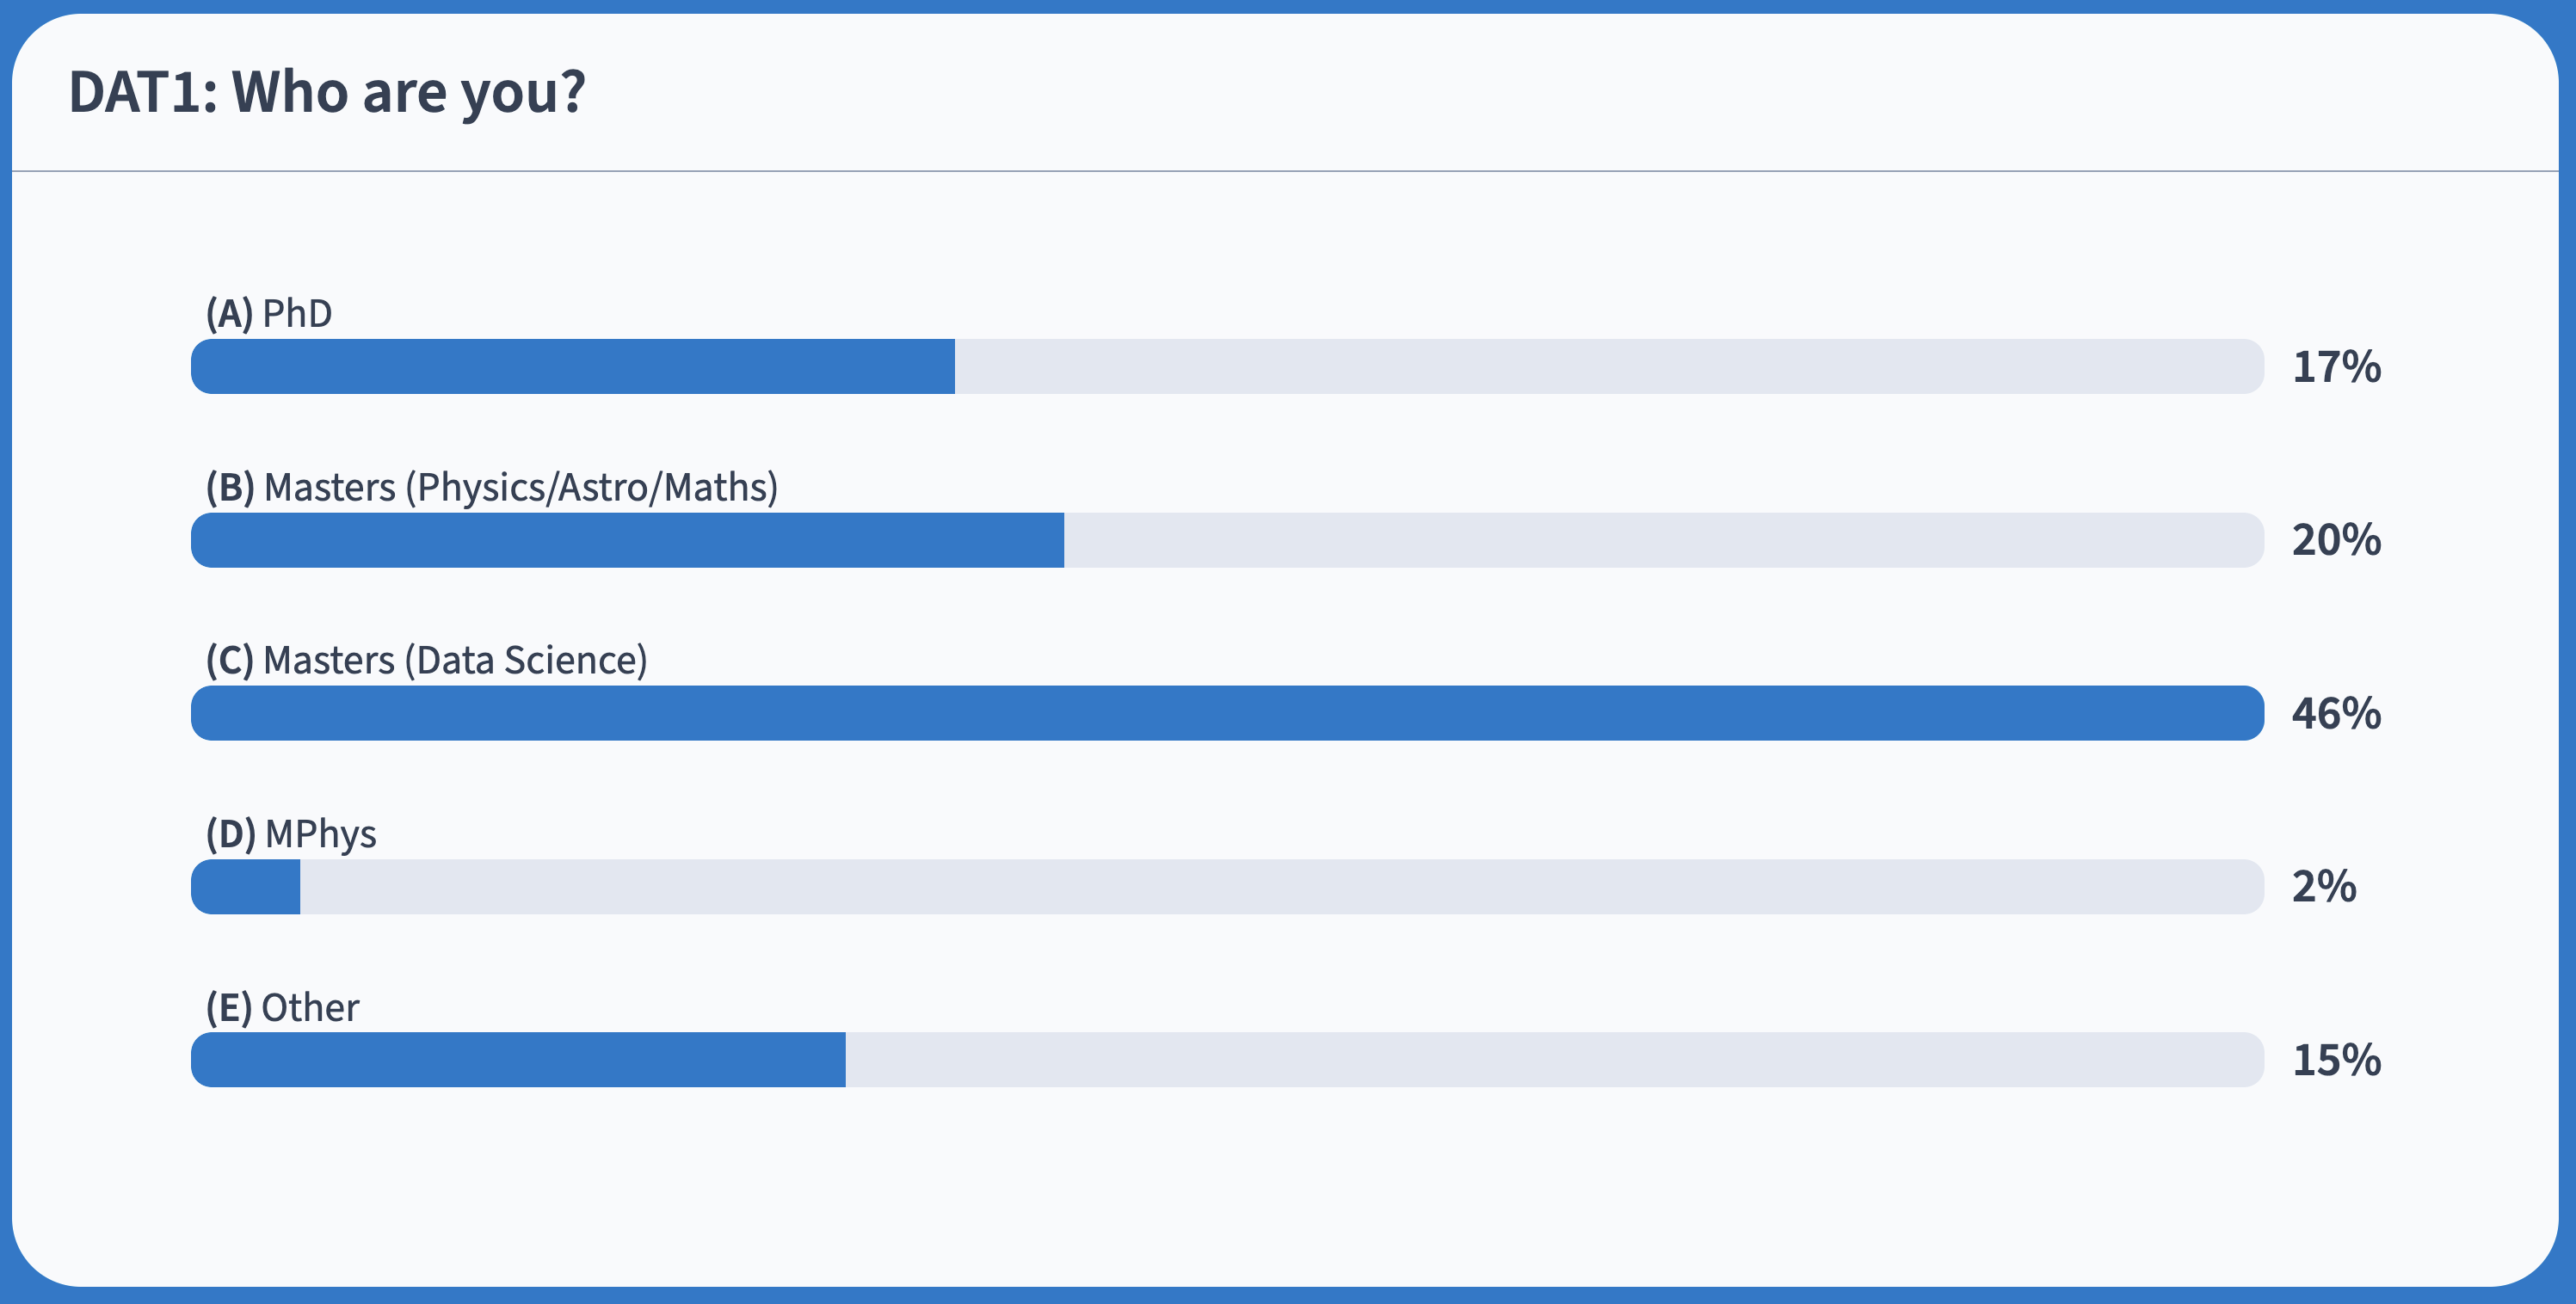
\includegraphics[scale=0.2]{DAT1-WhoAreYou}
\end{frame} 


\begin{frame}[fragile]{Polls from Monday}
\center
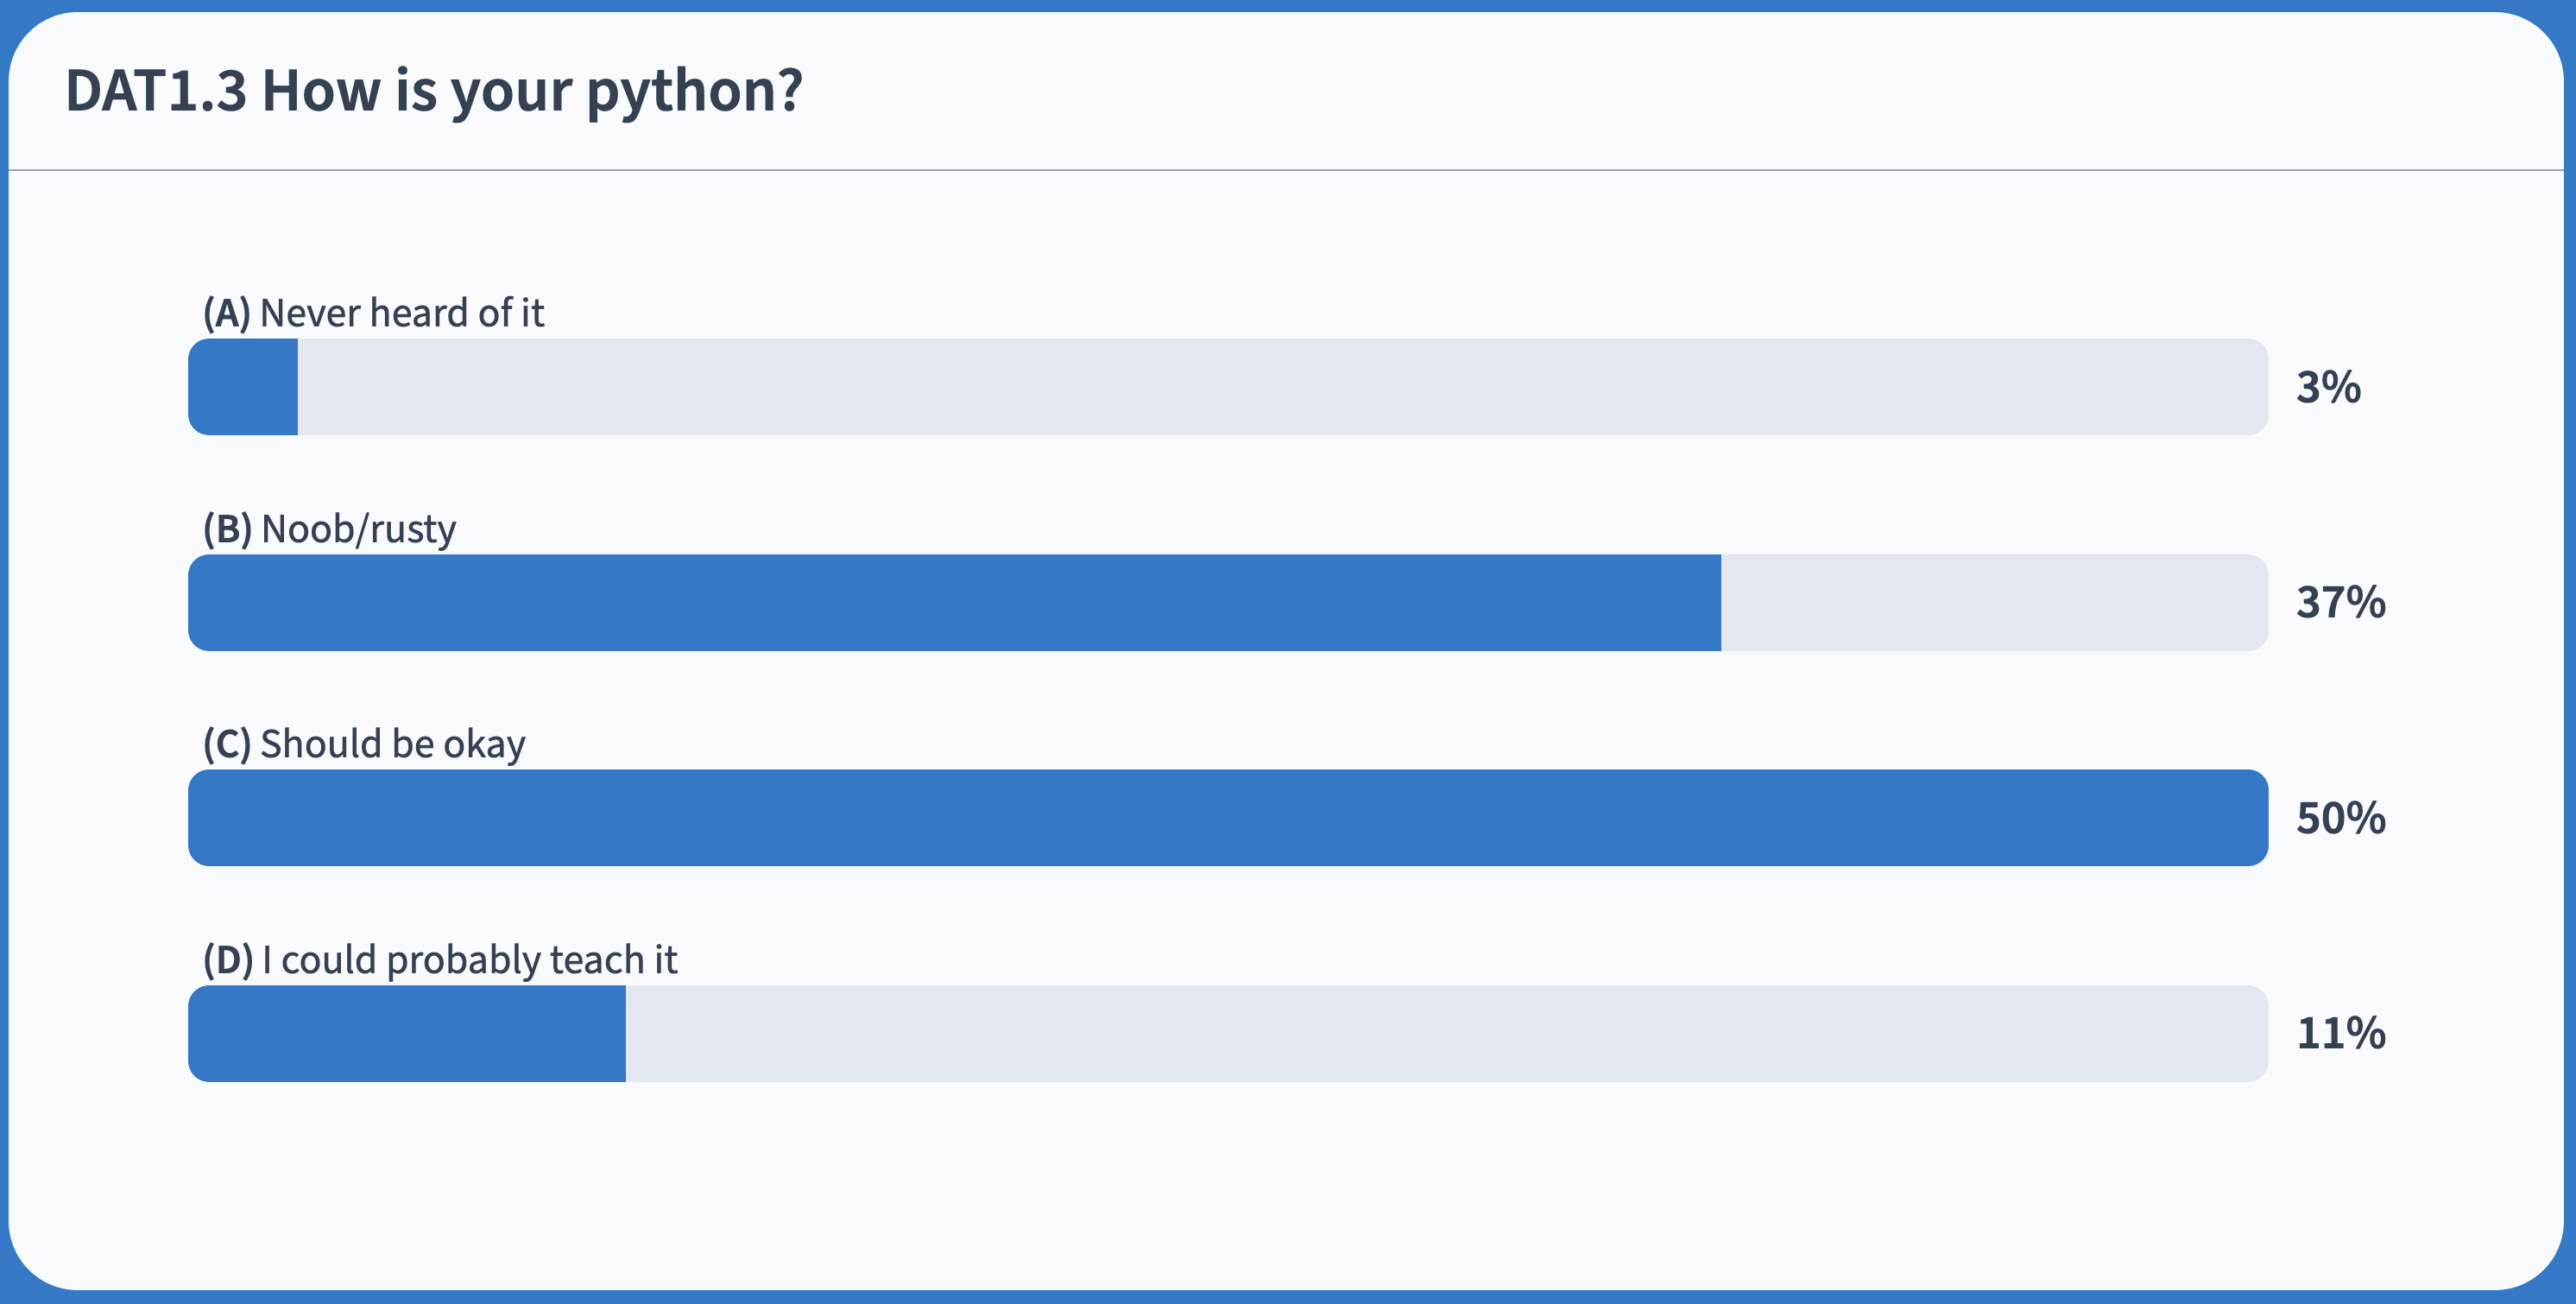
\includegraphics[scale=0.2]{DAT1-HowIsYourPython}
\end{frame} 


%\begin{frame}[fragile]{My Expectations}
%
%I do not expect the majority of you to be proficient in both mathematical tools and python.\\[1ex]
%
%Your proficiencies in either Math, Python are Random Variables. Your proficiencies in Math AND Python form a Joint PDF, which we will think about soon.\\[1ex]
%
%\begin{itemize}
%\item Maths no problem, focus on the python.\\
%\item Python no problem, focus on the math.\\
%\item Both a piece of cake, focus on other modules (but keep your eyes open).\\
%\item Both a problem, get comfy and start from the top. \\
%\end{itemize}
%
%\end{frame} 






% python
\begin{frame}[fragile]{Following with Python}

\begin{itemize}

\item[1] Install marimo as per instructions on the canvas Resources \& Prerequisites page.
\begin{minted}[bgcolor=LightGray]{bash}
pip install marimo
\end{minted}
\item[2] Open the canvas page for this week's material, and download the marimo notebook file \texttt{Probability.py}. 
\item[3] Run the notebook:
\begin{minted}[bgcolor=LightGray]{bash}
marimo edit Probability.py
\end{minted}
\end{itemize}

If you didn't install marimo yet, you can view the python here: \href{https://marimo.app/l/rub2g6}{https://marimo.app/l/rub2g6} - best if you don't edit it today :)\\[1ex]
\end{frame} 

 


\begin{frame}{Probability}
\large
\begin{itemize}
\item Notation\\[1ex]
\item Axioms\\[1ex]
\item Conditional Probability\\[1ex]
\item Bayes' Theorem\\[2ex]
\end{itemize}

I include a  small subset (ooh!) of terminology and symbols, for a more comprehensive list see eg \href{https://mathvault.ca/hub/higher-math/math-symbols/set-theory-symbols/}{here}.

\end{frame} 

\section*{Notation }

\begin{frame}[fragile]{Frequentist Probability}

Example Sets:\\[1ex]
$S = \{1,2,3,4,5,6,7,8,9,10\}$\\[1ex]
$A = \{2,4,6,8,10\}$\\[1ex]
$B = \{1,2,3,4\}$\\[1ex]

The \boo{Frequentist Probability} of A is written \boo{$P(A) = \dfrac{N_A}{N_S}$}:  \blu{the number of times A occurs in the sample divided by the number of possible outcomes in the sample.}. \\[1ex] 
Probabilities:\\[1ex]
$P(A) = N_A / N_S  = 0.5$\\[1ex]
$P(B) = N_B / N_S  = 0.4$\\[1ex]
$P(S) = N_S/N_S =1$\\[1ex]


\end{frame} 




\begin{frame}{Special Sets}

\center
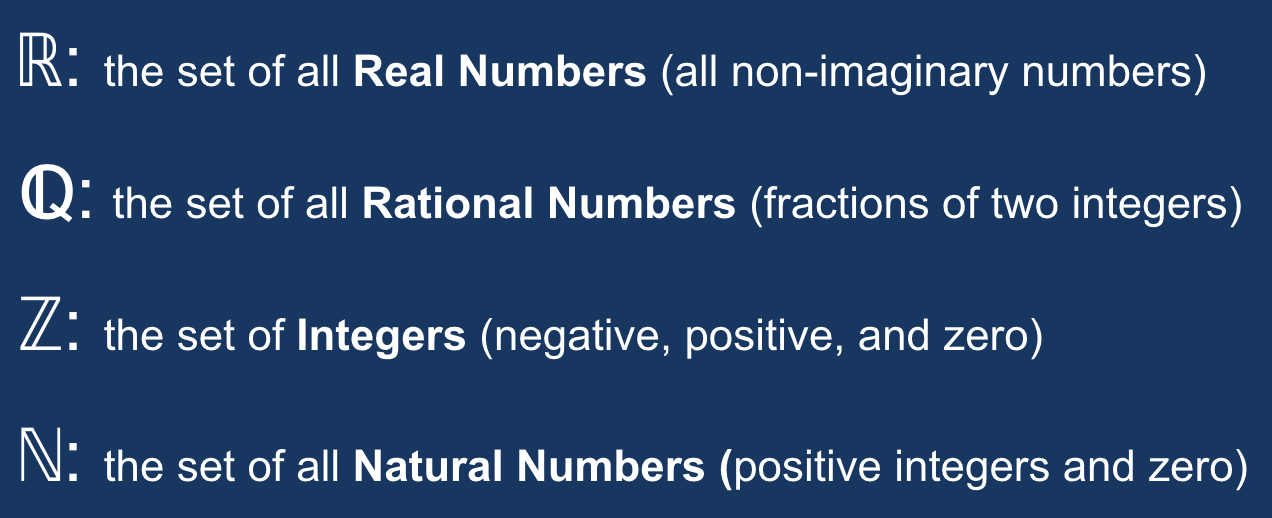
\includegraphics[scale=0.45]{SpecialSets}

\end{frame} 



%\begin{frame}{Sample Space}
%
%The \boo{Sample Space} is denoted by \boo{S}: \blu{the set of all possible outcomes}.\\[1ex]
%
%Note that a set of \textbf{outcomes} must be attached to some experiment.\\[1ex]
%
%%All Sample Spaces have satisfied
%\vspace{4cm}
%
%\end{frame} 


\begin{frame}[fragile]{Sample Space \& Subset}

The \boo{Sample Space} is denoted by \boo{S}: \blu{the set of all possible outcomes of some experiment or operation.}\\[3ex]

A \boo{Proper Subset} of S is written \boo{$A\subset S$}: A is a subset of S but A$\neq$S. \\[1ex] 
\blu{If A is a subset of S \textit{and} can be S, we use \boo{$A\subseteq S$}.}\\[3ex]

$S = \{1,2,3,4,5,6,7,8,9,10\}$\\[1ex]
$A = \{2,4,6,8,10\}$\\[1ex]
$B = \{1,2,3,4\}$\\[2ex]

\blu{A and B are proper subsets of S.}\\
\end{frame} 






\begin{frame}{Venn Diagrams}
Venn diagrams are helpful for visualising relationships. \\[1ex]
Here \boo{$A\subset S$} and \boo{$B\subset S$}.\\[1ex]
\vspace{0.5cm}
\center
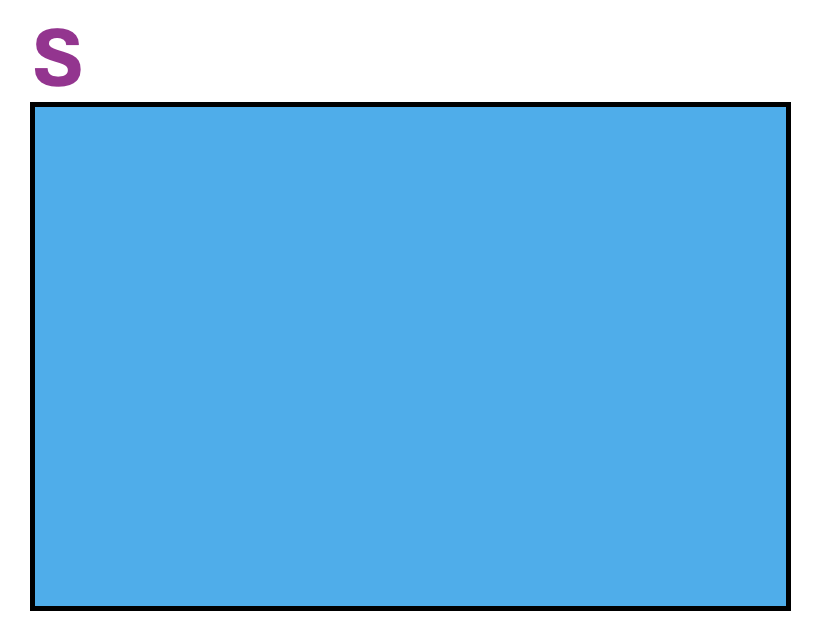
\includegraphics[scale=0.24]{S} 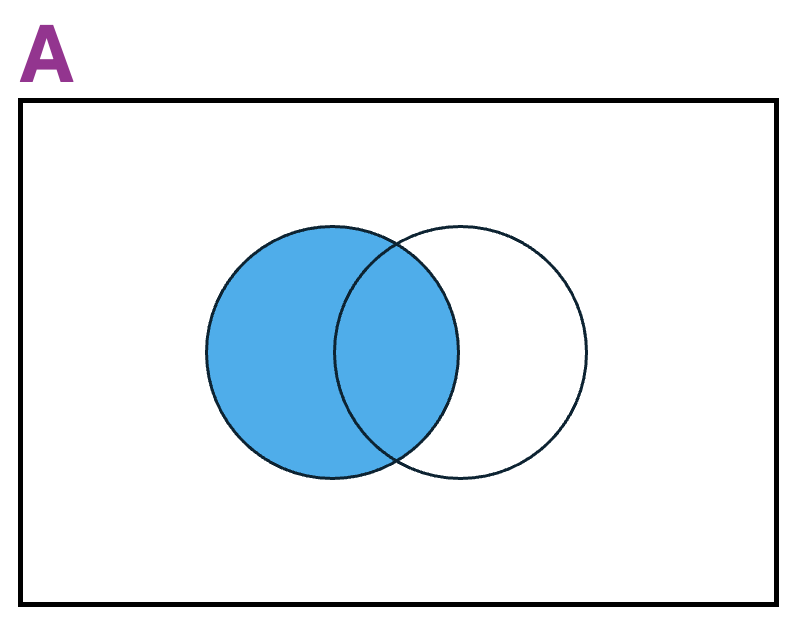
\includegraphics[scale=0.24]{A} 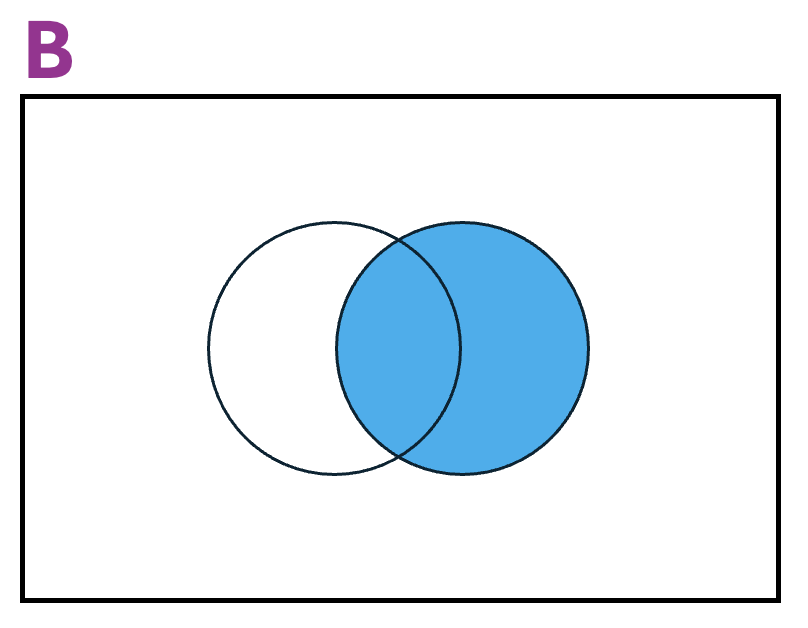
\includegraphics[scale=0.24]{B}

\end{frame}





\begin{frame}{Complement}


The \boo{Complement} of a set is denoted by a prime: \boo{A'}: this means `not A'.\\[1ex]
\blu{Other notations commonly used for the complement are: \boo{$A^{\complement}$},} \boo{$\overline{A}$ }, and several others.
\vspace{1cm}

\center
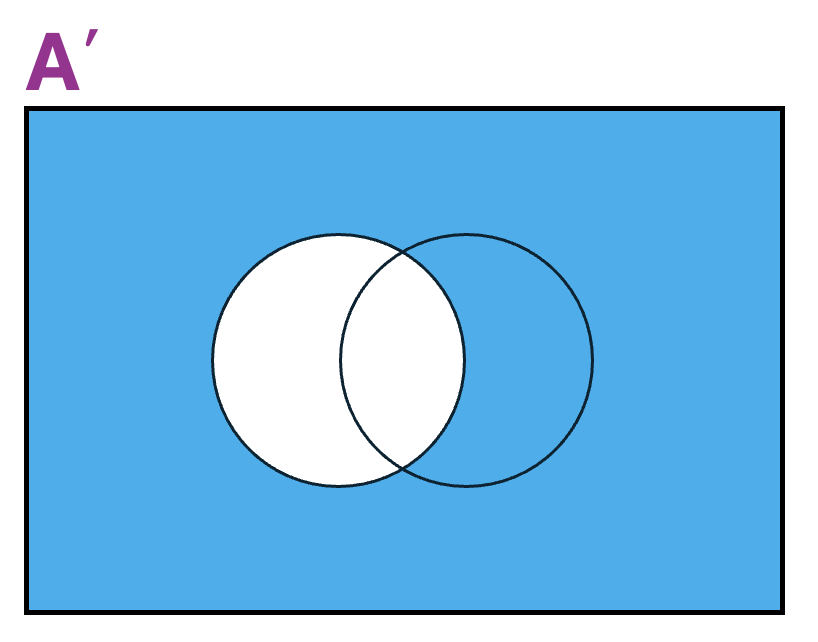
\includegraphics[scale=0.24]{NotA} 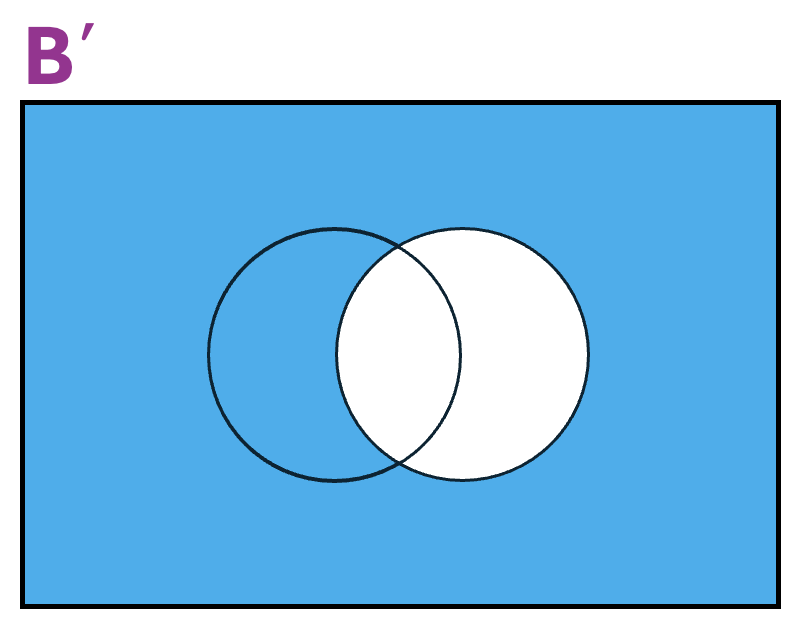
\includegraphics[scale=0.24]{NotB}

\end{frame} 



\begin{frame}[fragile]{Union}


The \boo{Union} of two sets is written: \boo{$A\cup B$}:  `either A, or B, or both'.\\[1ex]

\begin{multicols}{2}

$A = \{2,4,6,8,10\}$\\[1ex]
$B = \{1,2,3,4\}$\\[2ex]
$A\cup B = \{1,2,3,4,6,8,10\}$\\[2ex]


%\center
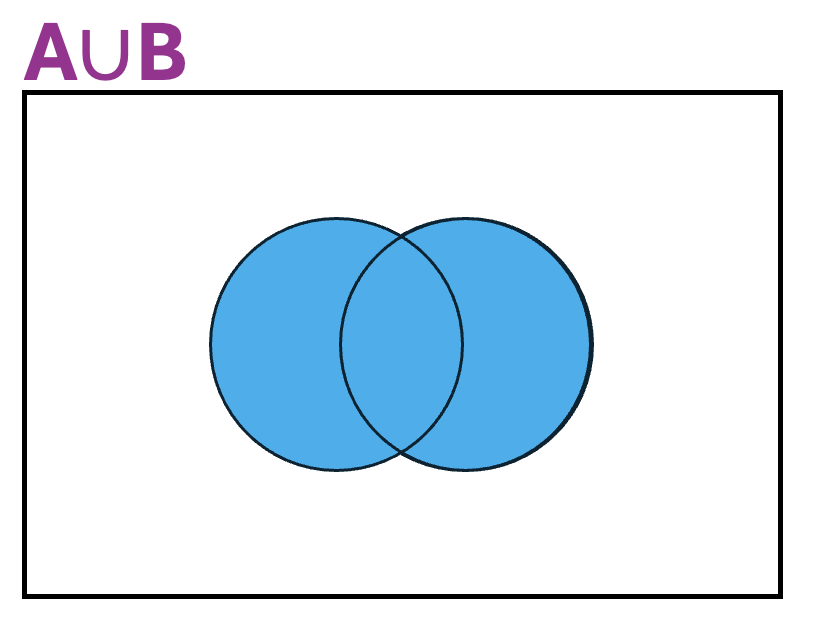
\includegraphics[scale=0.3]{AorB}


\end{multicols}
\end{frame} 


\begin{frame}[fragile]{Intersection}


The \boo{Intersection} of two sets is written: \boo{$A\cap B$}: ` both A and B'.\\[1ex]

\begin{multicols}{2}

$A = \{2,4,6,8,10\}$\\[1ex]
$B = \{1,2,3,4\}$\\[2ex]
$A\cap B = \{2,4\}$\\[2ex]


%\center
 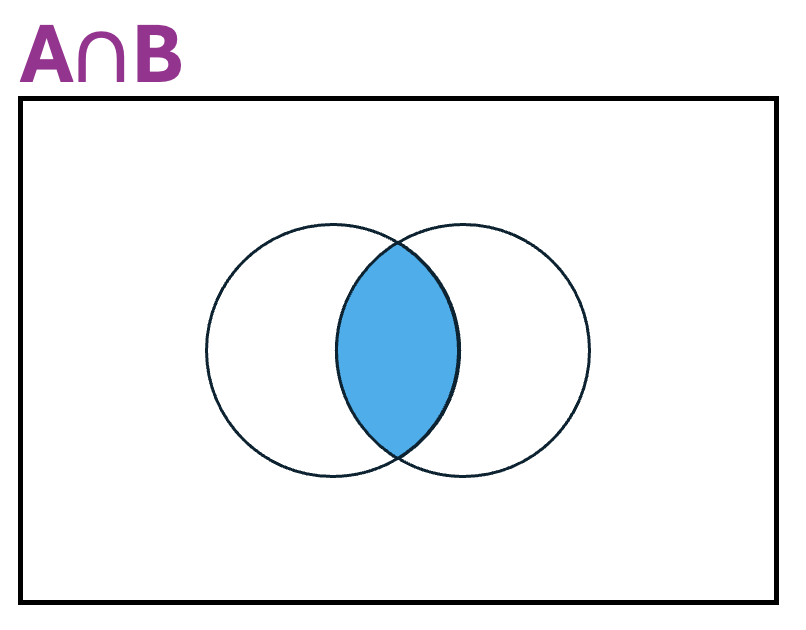
\includegraphics[scale=0.3]{AandB}

\end{multicols}
\end{frame} 


\section*{Axioms}


\begin{frame}[fragile]{Probability of Intersection}

The \boo{Probability of Intersection} $P(A\cap B)$: the probability that both A and B are true.\\[2ex]
This is zero when A and B are \boo{Disjoint} (no overlap: mutually exclusive)\\[1ex]

\begin{multicols}{2}

$P(A\cap B) =0 $ when $(A\cap B)' $\\[1ex]

\blu{
Our sets:\\
$A\cap B = \{2,4\}$\\[2ex]
$P(A\cap B) = 0.2$: $A$ and $B$ are not mutually exclusive.\\
}
  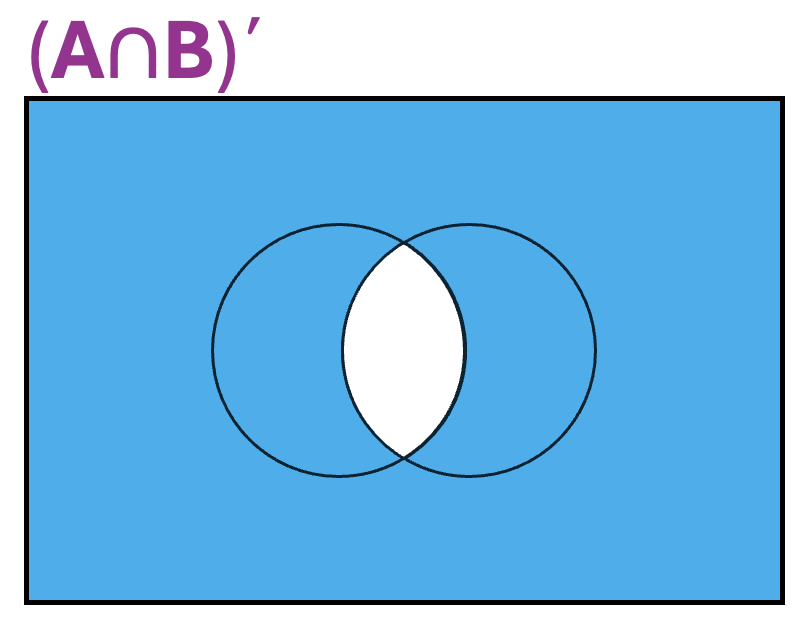
\includegraphics[scale=0.3]{NotAandB} 
  
  \end{multicols}
\end{frame} 


\begin{frame}[fragile]{Probability of  Union}

The \boo{Probability of Union} $P(A\cup B)$: the probability that either A or B or both are true.\\[2ex]
 
$P(A\cup B) =P(A)+P(B) - P(A\cap B)$.\\[2ex]

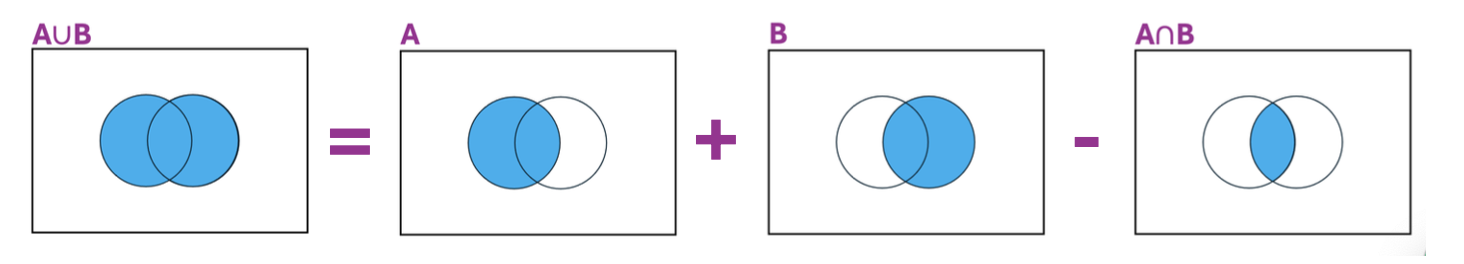
\includegraphics[scale=0.4]{Axiom3} 

\blu{
Our sets: $P(A\cup B) = 0.5 +0.4 - 0.2 = 0.7$.\\
} 
\end{frame} 



\begin{frame}[fragile]{The Kolmogorov Axioms}


1. The \boo{Non-Negativity Axiom} states that for all events A , $P(A) \geq 0\; $: \blu{ `the probability of any event A must be a real number greater than zero.'}.\\[1ex]

2.The \boo{Normalisation Axiom} states that  $P(S) =1$: the probability of the entire sample space is one.\\[1ex]

3.The \boo{Countable Additivity Axiom} states that  if A and B are mutually exclusive, $P(A\cup B) =P(A)+P(B)$: \blu{the probability of their union is the sum of their individual probabilities.}\\[1ex]

\end{frame} 


%\begin{frame}[fragile]{The Kolmogorov Axioms}





% \begin{minted}[bgcolor=LightGray]{python}
%# For our example sets (A and B are not mutually exclusive)
%P_AUB = len(AUB)/len(S) # 0.7
%P_A = len(A)/len(S) # 0.5
%P_B = len(B)/len(S) # 0.4
%P_AnB = len(AnB)/len(S) # 0.2
%\end{minted}

 
%\end{frame} 






\section*{Conditional Probability}

\begin{frame}[fragile]{Conditional Probability}

The \boo{Conditional Probability} $P(A | B) = \dfrac{P(A\cap B)}{P(B)}$\\[1ex]
\small
Example:\\
$A = \{2,4,6,8,10\}$\\
$B = \{1,2,3,4\}$\\
$A\cap B = \{2,4\}$\\

%Let B be our `reduced sample space'.\\
The number of elements in A and B is $N(A \cap B)$\\
\blu{The proportion of A in B is $\dfrac{N(A\cap B)}{N(B)}$}\\
Relative to the original Sample Space S this is: $\dfrac{N(A\cap B)/N(S) }{N(B)/N(S)}$\\
\blu{These are probabilities: $\dfrac{P(A\cap B)}{P(B)}$}\\
Given that we demand the element must exist in B, this is the probability of finding it in A.\\

\end{frame} 



\begin{frame}[fragile]{Conditional Probability}

The \boo{Conditional Probability} $P(A | B) = \dfrac{P(A\cap B)}{P(B)}$.\\[2ex]

If A and B are \textbf{Independent}, the conditional probability $P(A | B)  = P(A) $.\\[2ex]

This is because independence means that B has no effect on A and vice versa.\\[2ex]

\blu{
Our example sets are independent. $P(A| B) = P(A) = 0.5$.\\
} 

\end{frame} 


\begin{frame}[fragile]{Using the Conditional Probability}
It is common to use conditional probabilities when we have a set of outcomes (A) and a set of choices (B).\\[1ex]

The Conditional Probability $P(A | B) = \dfrac{P(A\cap B)}{P(B)}$  then gives us an answers to the question: \blu{If I choose $B_i$, what is the probability of the outcome $A_i$?}\\[2ex]
%How does this differ from $P(B | A) = \dfrac{P(B\cap A)}{P(A)}$?\\[1ex]
Conditional Probability looks harmless enough, but can have some counter-intuitive results illustrated very well in the \textbf{Monty Hall Problem}, which you will look at in your homework/workshop.\\[1ex]


\end{frame} 


\begin{frame}[fragile]{The Multiplication Rule}

Rearrange the Conditional Probability:\\

$P(A | B) = \dfrac{P(A\cap B)}{P(B)} \therefore  P(A\cap B) = P(A | B) P(B) $  \\[1ex]
%
%This is a very useful rearrangement of the conditional probability. If A and B are independent, it simplifies to:\\[1ex]

\boo{The Multiplication Rule}: $P(A\cap B) = P(A) P(B) $: \blu{If A and B are independent, the probability of the intersection of A and B is equal to the product of their individual probabilities.}\\[1ex]

Example: I roll a dice twice and get two sixes:\\[1ex]
$P(six \cap six) = P(six) P(six) = \dfrac{1}{6} \dfrac{1}{6}  = \dfrac{1}{36}$

\end{frame} 

\begin{frame}[fragile]{The Total Probability}

Referring to the picture below with $N=4$ disjoint sets $B_i$ intersecting with A, we can see that $P(A) = \sum \limits_i^4 P(A\cap B_i)$.\\[2ex]

\center
 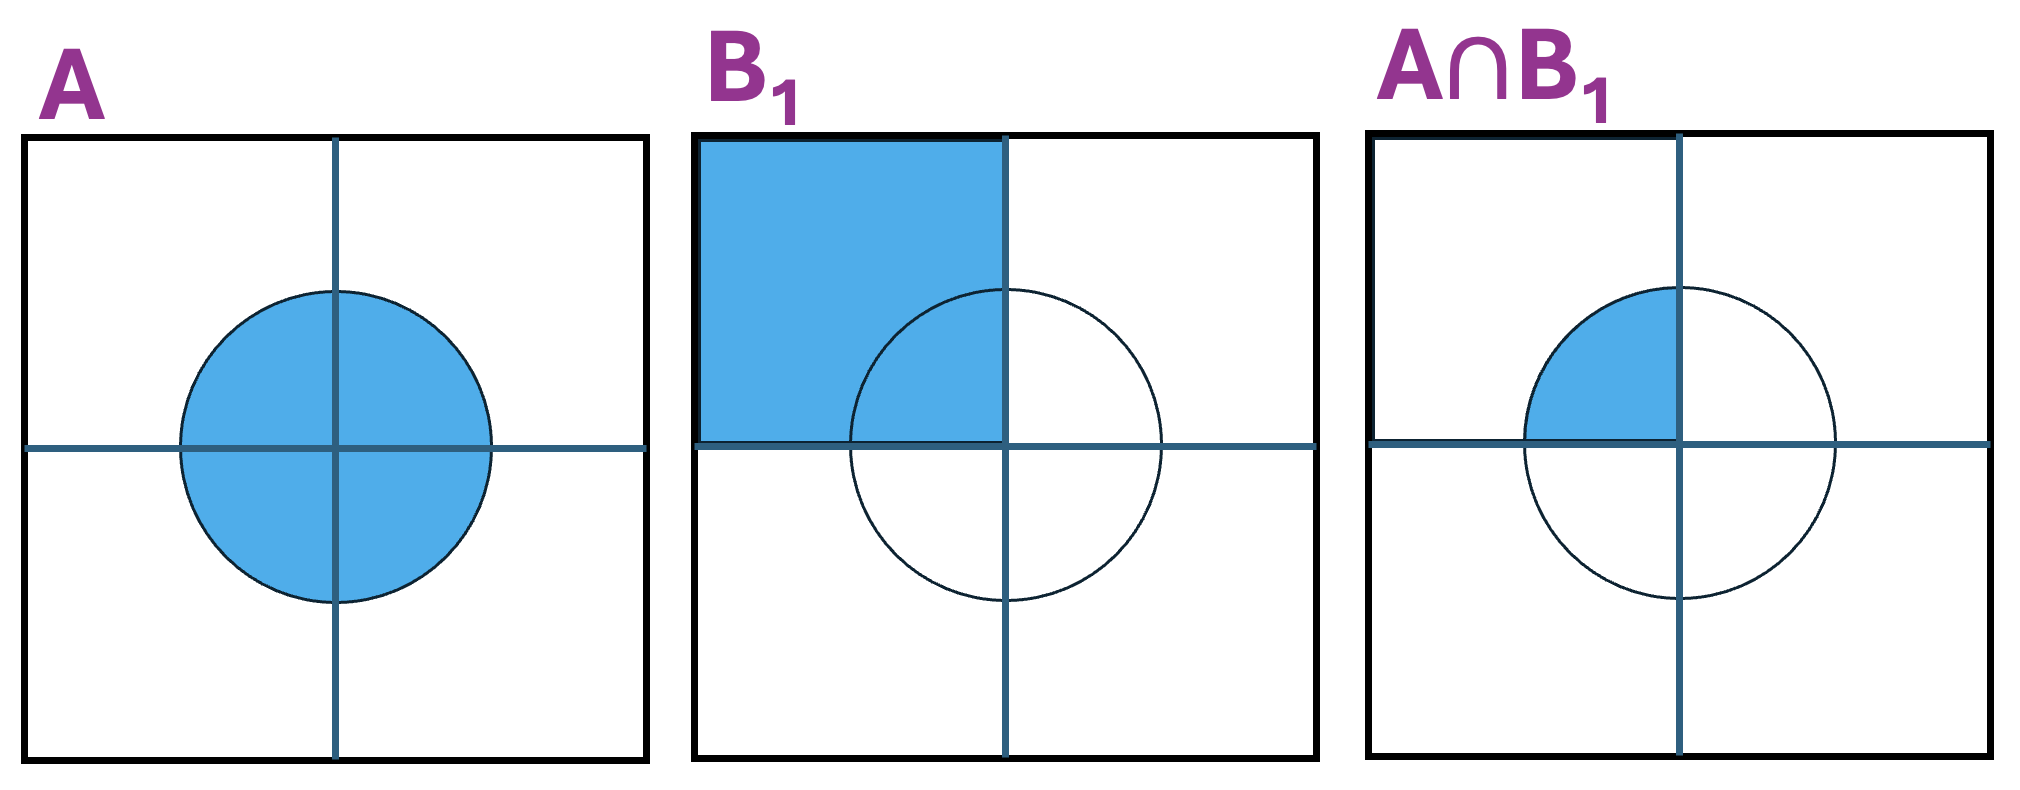
\includegraphics[scale=0.3]{AandB1} 
 
\end{frame} 


\begin{frame}[fragile]{The Total Probability}

From our example: $P(A) = \sum \limits_i^N P(A\cap B_i)$.\\[2ex]
Comparing with the Conditional: $P(A\cap B) = P(A | B) P(B) $\\[4ex]
The \boo{Law of Total Probability} is written:\\[1ex]
 $P(A) = \sum \limits_i^N P(A | B_i) P(B_i)$.\\[3ex]
 
 \blu{This may seem a bit contrived, but we will see soon that it is useful.}
\end{frame} 




\section*{Bayes' Theorem}

\begin{frame}[fragile]{Bayes' Theorem}

We have the \boo{Conditional Probability}:\\[2ex]
$P(A\cap B) = P(A | B) P(B)$,   \blu{therefore}  $P(B\cap A) = P(B | A) P(A)$\\[4ex]
%Note that $\boo{P(A\cap B)} = \boo{P(B\cap A)}$:
\boo{Bayes' Theorem} simply combines these: \\[2ex]%uses $ P(B\cap A) = P(A\cap B)$:\\[2ex]
\center
$P(A | B) = 
\dfrac{
P(B|A)P(A)
}
{
P(B)
}
$\\[1ex]
% \center
%  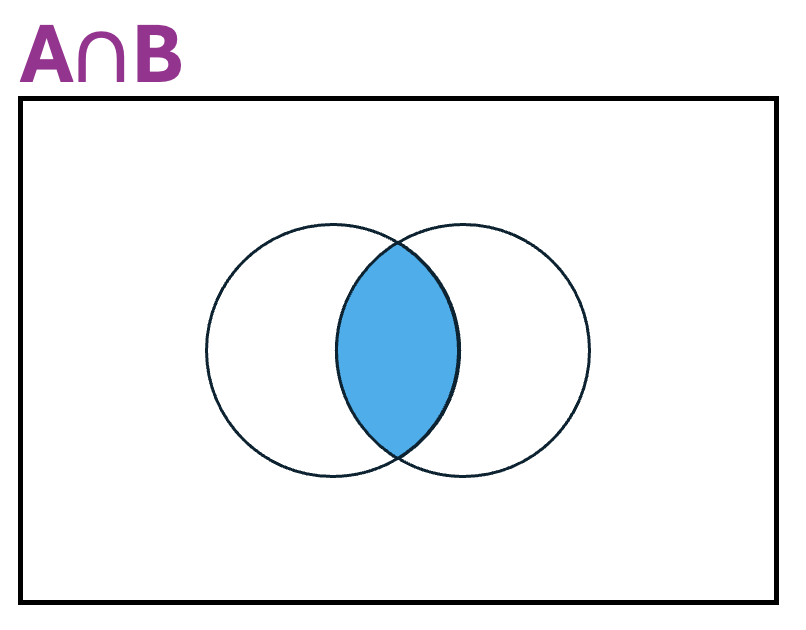
\includegraphics[scale=0.22]{AandB} 
\blu{On the left we have P of A given B, and on the right P of B given A}
\end{frame} 

\begin{frame}[fragile]{Bayes' Theorem for our sets}

$P(A | B) = 
\dfrac{
P(B|A)P(A)
}
{
P(B)
}
$\\[1ex]

$P(A| B) = P(A) = 0.5$\\
$P(B| A) = P(B) = 0.4$\\[3ex]
The so-called theorem tells us nothing! \frownie{} \\[1ex]


Bayes' Theorem gets interesting when we consider that it applies to \textbf{any sets $A$ and $B$ that satisfy Kolmogorov's Axioms}.\\[2ex]


% \center
%  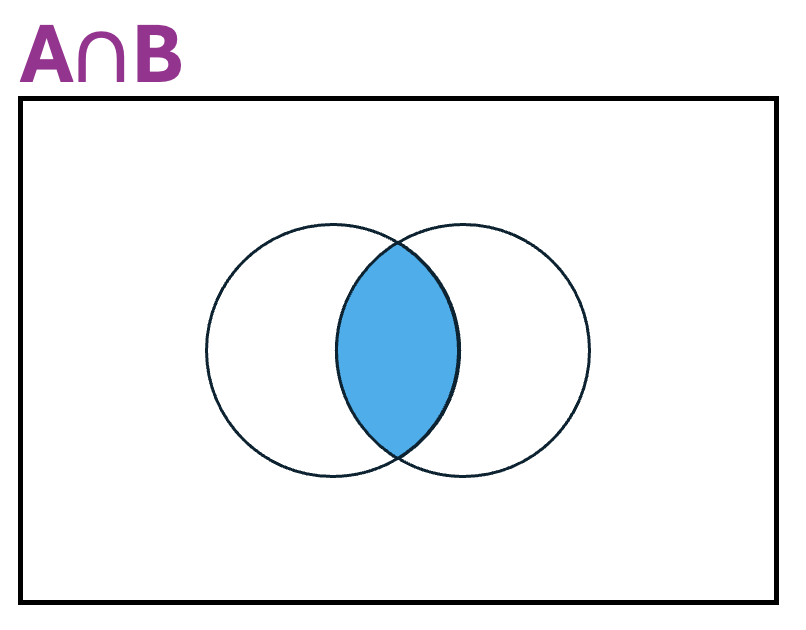
\includegraphics[scale=0.22]{AandB} 

\end{frame} 




\begin{frame}[fragile]{Bayes' Theorem for a Hypothesis}

Our Hypothesis is H, for example `My dog is a good boy'.\\[1ex]
Our Data is X, for example `Test results from behaviour school'.\\[1ex]

$P(H | X) = \dfrac{ P(X|H) P(H) } { P(X) } $\\[1ex]

$P(H | X)$: \blu{Probability of a Hypothesis, given the Data}\\[1ex]
$P(X | H)$: \blu{ Likelihood of the Data, given a Hypothesis}\\[1ex]
$P(X)$: \blu{ Probability of the Data}\\[1ex]
$P(H)$: \blu{ Probability of the Hypothesis}\\[1ex]

\end{frame} 


\begin{frame}[fragile]{The Prior Probability $P(H) = \pi(H)$}

Recall, the \boo{Frequentist Probability} of A is written \boo{$P(A) = \dfrac{N_A}{N_S}$}:  the number of times A occurs in the sample divided by the number of possible outcomes in the Sample Space. \\[1ex] 

The probability of my hypothesis $P(H)= \dfrac{N_H}{N_S}$: the sample space S has to be that of all Hypotheses.\\[1ex]

This is called the \boo{Prior Probability} because it requires some prior knowledge. In this case, the question answered by the prior would be \blu{`What percentage of dogs are good?'} This is very special so we give it a special symbol,  $P(H) = \pi(H)$. Notice that it has nothing to with the test. \\[1ex]

%\small
%\textcolor{red}{*$\pi(H)=1$. They are all good. This is my prior.}
\end{frame} 


\begin{frame}[fragile]{Bayes with Prior $ \pi(H)$}

Bayes is now:\\[1ex]
$P(H | X) = \dfrac{ P(X|H) \pi(H) } { P(X) } $\\[1ex]

Using the \boo{Law of  Total probability}  $P(A) = \sum \limits_i^N P(A | B_i) P(B_i)$, we can write Bayes as:\\[1ex]

$P(H_i | X) = \dfrac{ P(X | H_i) \pi(H_i) } { \sum\limits_i^N P(X | H_i) \pi(H_i)}$ \\[1ex]

Where $H_i$ is my hypothesis, and the sum in the denominator is over all possible hypotheses.



\end{frame} 



\begin{frame}[fragile]{Bayes' Theorem: Useful Form}


$P(H_i | X) = \dfrac{ P(X|H_i) \pi(H_i) } {  \sum\limits_i^N P(X | H_i) \pi(H_i) } $\\[2ex]
$P(H_i | X)$: \boo{ Posterior Probability} of my Hypothesis being correct, given the Data.\\[2ex]
$P(X | H_i)$: \boo{ Likelihood} of the Data, given my Hypothesis is correct\\[2ex]
$\pi(H_i)$: \boo{ Prior Probability} of my hypothesis $H_i$\\[2ex]
Denominator= $\pi(X)$: \boo{ Total probability} of the Data given any hypothesis.\\[2ex]


\end{frame} 


\begin{frame}[fragile]{Bayes' Theorem is not 'Bayesian' - it is just math}

I mentioned there are two philosophies: Bayesian and Frequentist. Using Bayes' theorem does not make one a Bayesian.\\[1ex]

%Remember we have used the frequentist probability in constructing Bayes.\\[1ex]

A frequentist would happily use Bayes' theorem, but \textbf{not to answer the question of whether my dog is good (or any other hypothesis)}. To a frequentist, a hypothesis is either right or wrong and does not have an associated Probability Distribution.\\[1ex]

The frequentist approach to answering this question would be to construct a \textbf{Likelihood} function $ \mathcal{L}(x|\theta)$ based only on the data $x$, and to minimise it for a variety of different hypotheses in order to find the `best' one.
%I can tell them unequivocally that $\pi(Hi) =1$ in this case\textcolor{red}{*}, but in that case a frequentist would not need to look at the data again. They would, however, question the methods used to calculate $\pi(Hi) =1$ in the first place. \\[1ex]

\small
%\textcolor{red}{* This is a joke about how much I love dogs.}

\end{frame} 



\begin{frame}{Thanks For Your Time}
\center
\Huge
Fin.
\end{frame}





\end{document}
